\documentclass[11pt,letterpaper,titlepage]{article}

\usepackage{geometry}
\geometry{left=2cm,right=2cm,top=2cm,bottom=3cm}

\usepackage{setspace}
\onehalfspacing

\usepackage{multicol}
\setlength{\columnsep}{3em}

\usepackage{booktabs}

\usepackage[table,x11names]{xcolor}

\usepackage{multirow}

\usepackage{pgfgantt}

\usepackage{listings}

\usepackage{xcolor}
\definecolor{vgreen}{RGB}{104,180,104}
\definecolor{vblue}{RGB}{49,49,255}
\definecolor{vorange}{RGB}{255,143,102}

\lstdefinestyle{C-style}
{
    language=C,
    basicstyle=\small\ttfamily,
    keywordstyle=\color{vblue},
    identifierstyle=\color{black},
    commentstyle=\color{vgreen},
    % numbers=left,
    numberstyle=\tiny\color{black},
    numbersep=11pt,
    tabsize=4,
    moredelim=*[s][\colorIndex]{[}{]},
    literate=*{:}{:}1
}

\lstdefinestyle{txt-style}
{
    basicstyle=\small\ttfamily,
    % numbers=left,
    numbersep=11pt,
    tabsize=4,
    moredelim=*[s][\colorIndex]{[}{]},
    literate=*{:}{:}1
}

\usepackage{tikz}
\usetikzlibrary{shapes.geometric, arrows, positioning, fit,calc}
\newcommand*\circled[1]{\tikz[baseline=(char.base)]{
            \node[shape=circle,draw,inner sep=1pt] (char) {#1};}}
            
\usepackage{hyperref}
\hypersetup{
    colorlinks,
    citecolor=black,
    filecolor=black,
    linkcolor=black,
    urlcolor=black
}

\usepackage{pifont}

\usepackage[toc,page]{appendix}

\pagestyle{empty}
\usepackage{tikz}
\usetikzlibrary{shapes.geometric, arrows}

\usetikzlibrary{mindmap,trees}
\usepackage{verbatim}

\usepackage{indentfirst}
\setlength{\parindent}{2em}

\usepackage{listings}

\usepackage{chngcntr}
\counterwithin{section}{part}
\renewcommand\thesection{\arabic{section}}

\usepackage{graphicx}

\usepackage{subcaption}

\usepackage{fancyhdr}

\pagestyle{fancy}
\lhead{}
\rhead{}
\lfoot{ECEN 749 Section 601 Lab 4}
\cfoot{\thepage}
\rfoot{@Lei Wang (Wilson)}
\renewcommand{\headrulewidth}{0pt}
\renewcommand{\headwidth}{\textwidth}
\renewcommand{\footrulewidth}{0.4pt}
\newcommand{\RomanNumeralCaps}[1]
    {\MakeUppercase{\romannumeral #1}}

\makeatletter
\newcommand*\@lbracket{[}
\newcommand*\@rbracket{]}
\newcommand*\@colon{:}
\newcommand*\colorIndex{%
    \edef\@temp{\the\lst@token}%
    \ifx\@temp\@lbracket \color{black}%
    \else\ifx\@temp\@rbracket \color{black}%
    \else\ifx\@temp\@colon \color{black}%
    \else \color{vorange}%
    \fi\fi\fi
}
\makeatother

\usepackage{trace}

\begin{document}

\begin{titlepage}
  \centering
	{\scshape\large Texas A\&M University \par}
	\vspace{1cm}
	{\scshape\Large Department of Electrical and Computer Engineering \par}
	\vspace{4cm}
    \vspace{0.5cm}
	{\huge\bfseries ECEN 749 Microprocessor System Design\par}
	\vspace{4cm}
	{\Large Lab 4 Report (Section 601)\par}
	\vspace{1cm}
	{\Large Student: Lei Wang (Wilson)\par}
	\vspace{1cm}
	{\Large UIN: 829009485\par}
	\vspace{1cm}
	{\Large Instructor: Dr. Paul V. Gratz\par}
	\vspace{4cm}
	\vfill

  % Bottom of the page
	{\large Submitted: February 18th, 2020 \par}

\end{titlepage}

\newpage

\tableofcontents{}

\newpage

\part{Introduction}

The purpose of the lab is to teach students how to run Linux on the ZYBO Z7-10 board. The process involves creating the block diagram design, generating the \textbf{BOOT.bin} file, compiling the Linux kernel, configuring the devicetree and making the ramdisk image. All the files generated are transferred to a micro-SD card and the FPGA board is configured to boot from the micro-SD card. Picocom is used to observe the output.

\part{Procedure}


\newpage

\part{Results}

The first few trials did not succeed, even after checking the block design and re-making the ramdisk, etc. It turned out the micro-SD card was written before by others and deleting files on micro-SD cards could not purge the existence of other files. During booting stage, errors such as corrupted ramdisk image or missing ramdisk image may show up. Formatting the micro-SD card with FAT file system before transferring files solves the problem. A successful boot can be observed from Picocom:

\begin{figure}[ht]
    \centering
    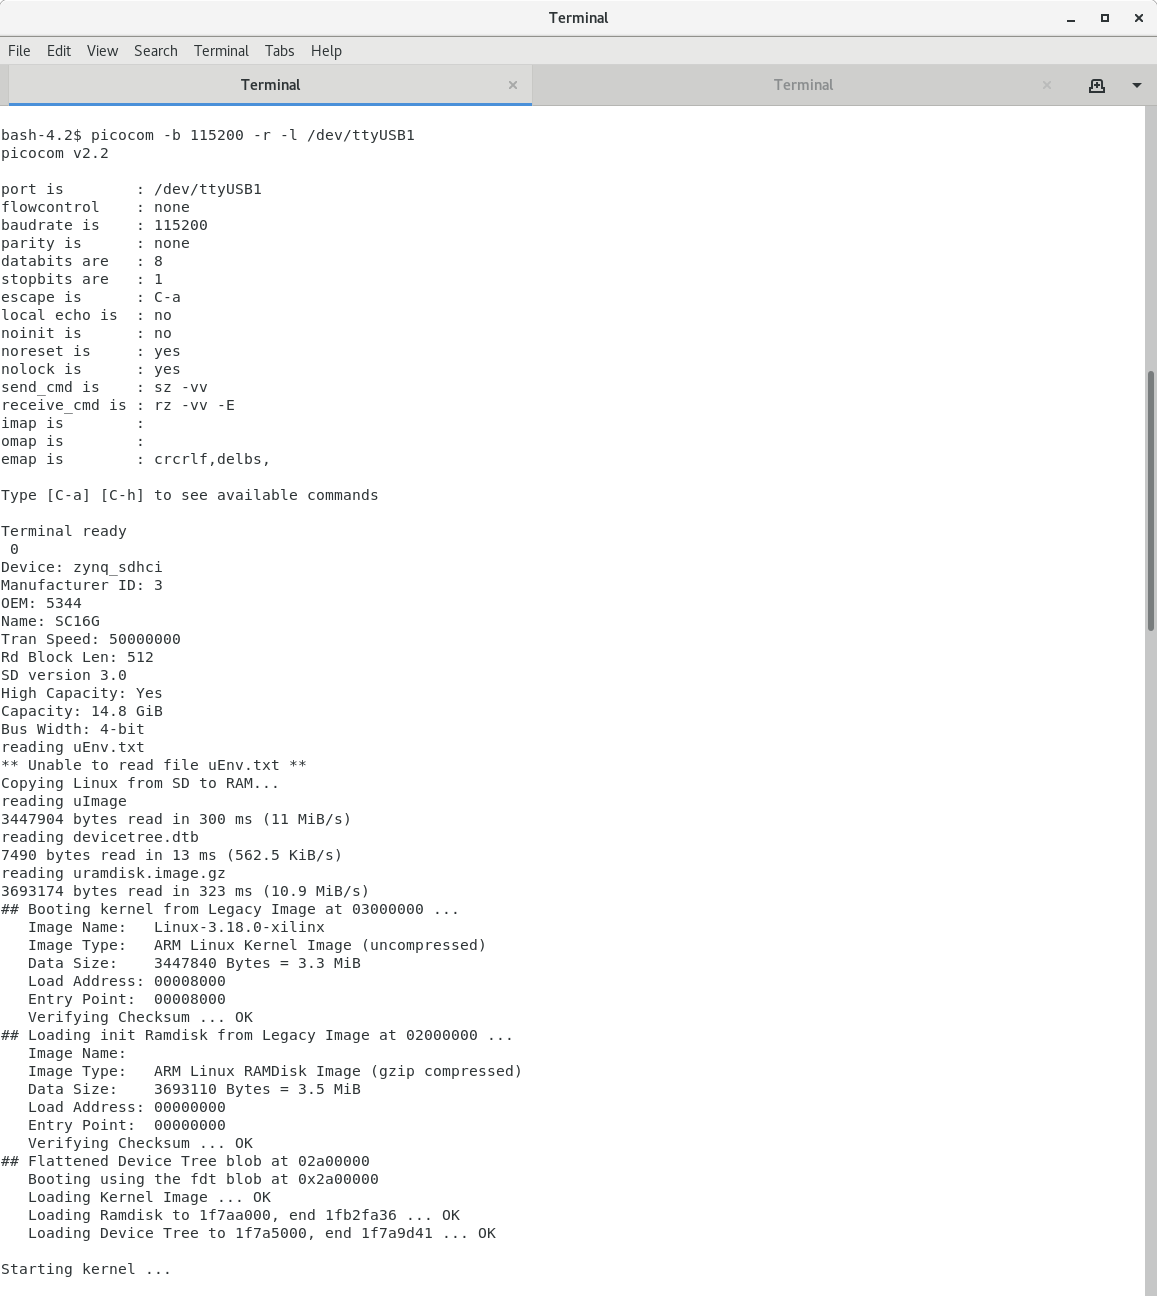
\includegraphics[width=0.85\textwidth]{boot_1.png}
    \caption{Booting Linux on ZYBO Z7-10 Picocom output 1/4.}
\end{figure}

\newpage

\begin{figure}[h!]
    \centering
    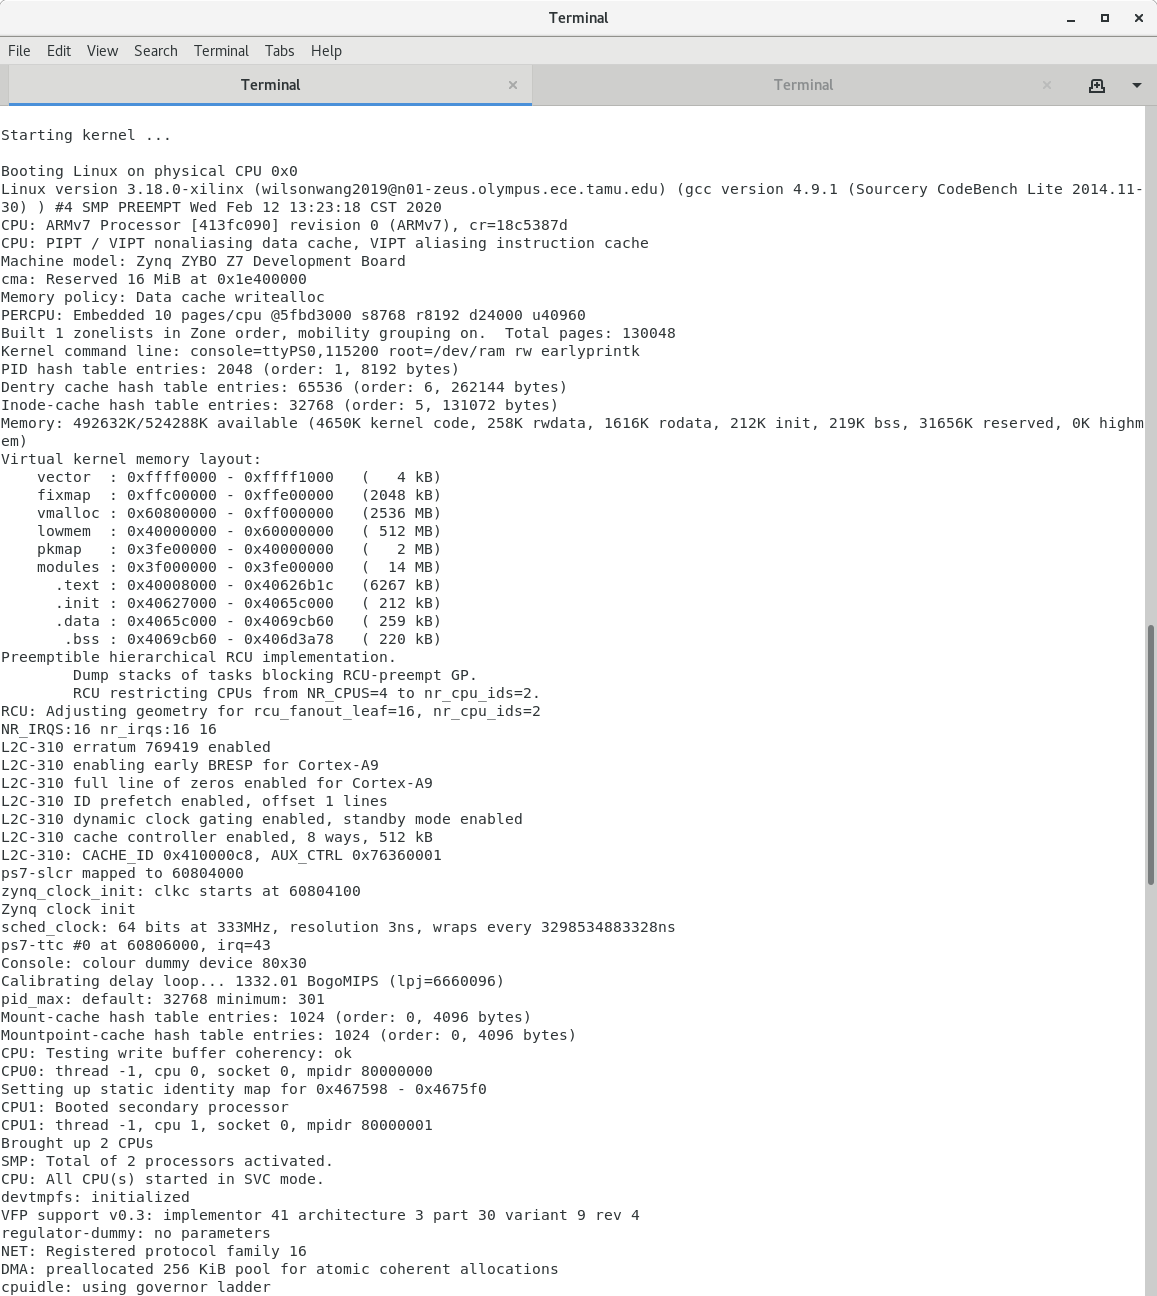
\includegraphics[width=\textwidth]{boot_2.png}
    \caption{Booting Linux on ZYBO Z7-10 Picocom output 2/4.}
\end{figure}

\newpage

\begin{figure}[h!]
    \centering
    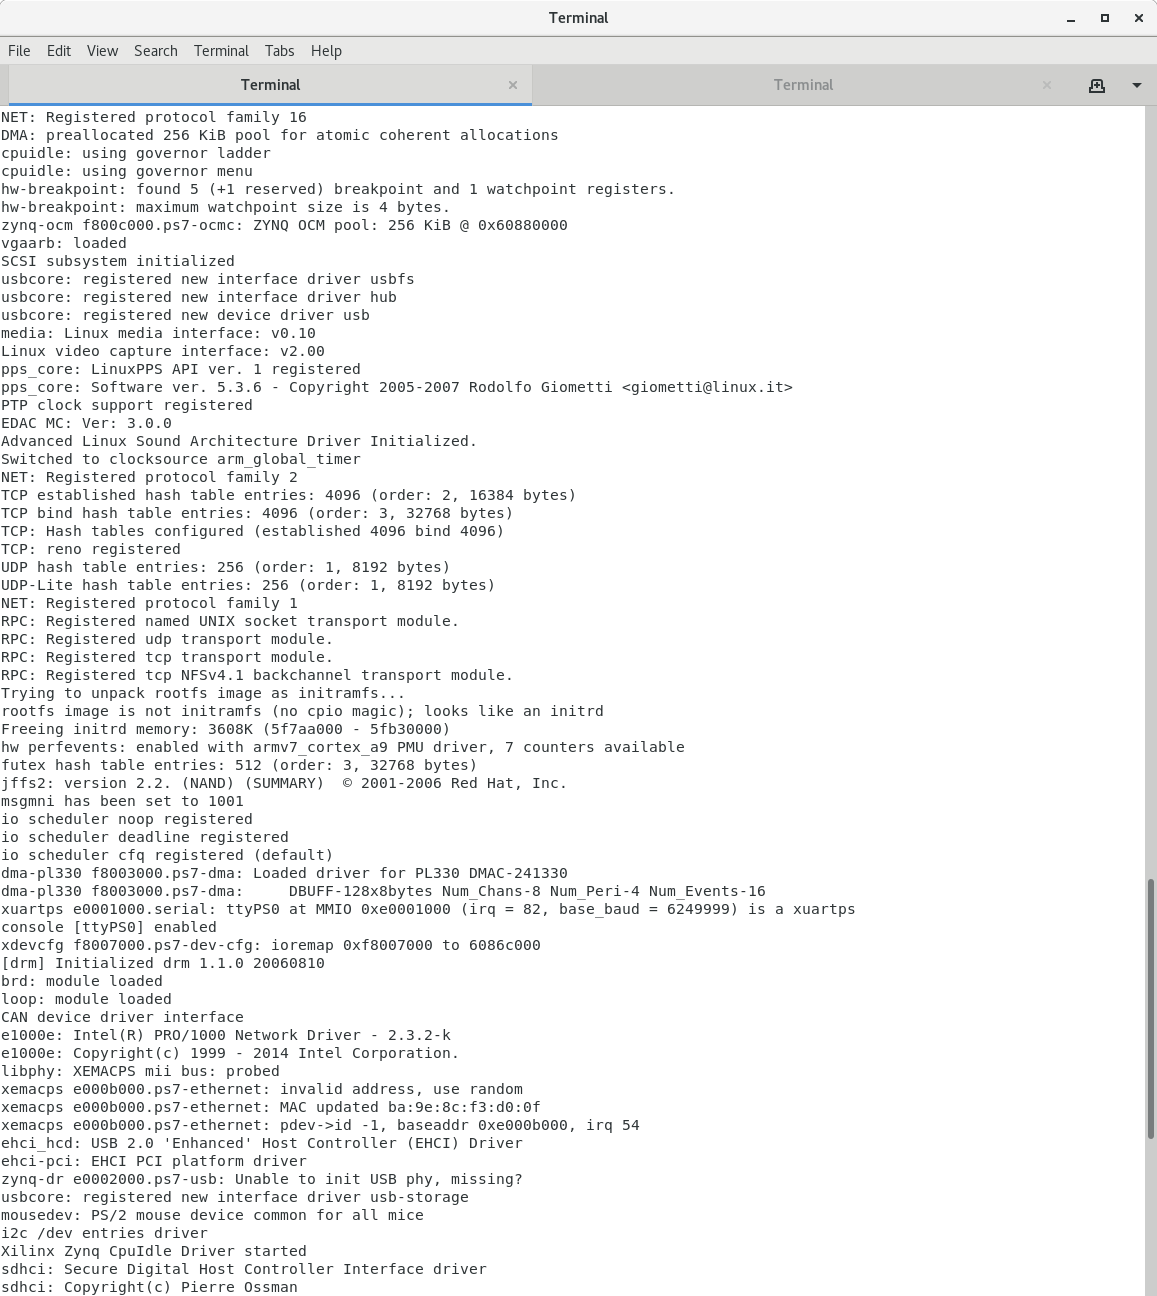
\includegraphics[width=\textwidth]{boot_3.png}
    \caption{Booting Linux on ZYBO Z7-10 Picocom output 3/4.}
\end{figure}

\newpage

\begin{figure}[h!]
    \centering
    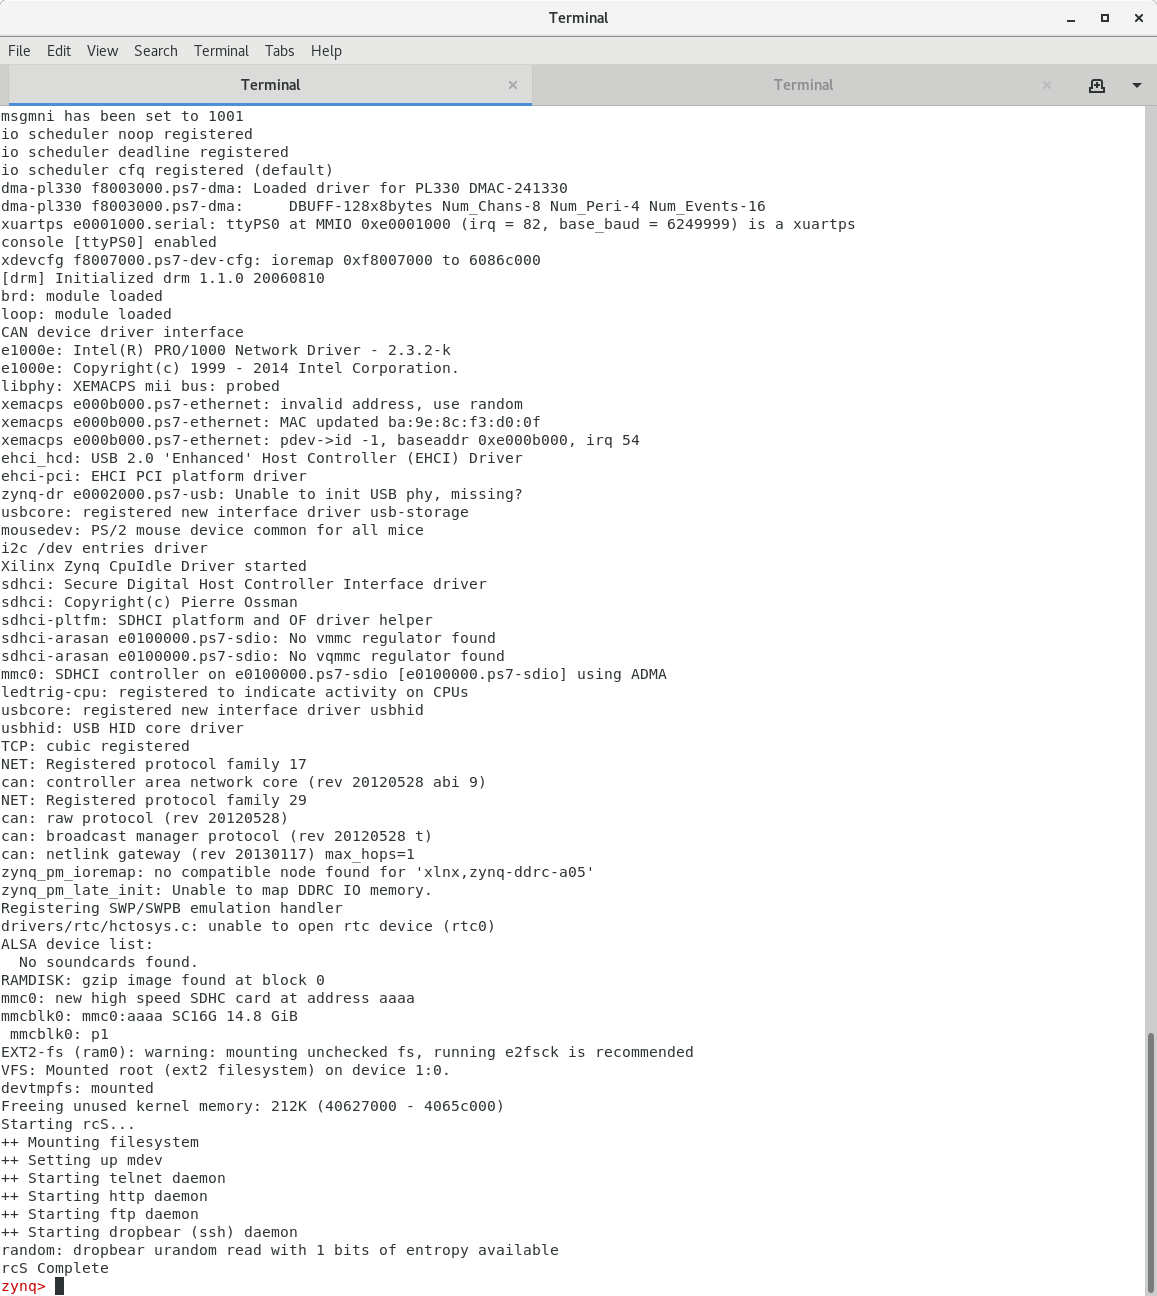
\includegraphics[width=\textwidth]{boot_4.png}
    \caption{Booting Linux on ZYBO Z7-10 Picocom output 4/4.}
\end{figure}

\newpage

\part{Conclusion}

\textbf{Q: Compared to lab 3, the lab 4 microprocessor system shown in Figure 1 has 512 MB of SDRAM. However, our system still includes a small amount of local memory. What is the function of the local memory? Does this ``local memory'' exist on a standard motherboard? If so, where?}

A: In the 

\textbf{Q: After your Linux system boots, navigate through the various directories. Determine which of these directories are writable. (Note that the man page for ``ls'' may be helpful). Test the permissions by typing ``touch $<$filename$>$'' in each of the directories. If the file, $<$filename$>$, is created, that directory is writable. Suppose you are able to create a file in one of these directories. What happens to this file when you restart the ZYBO Z7-10 board? Why?}

A: Running \verb|ls -al| in Picocom gives the following result:

\begin{figure}[ht]
    \centering
    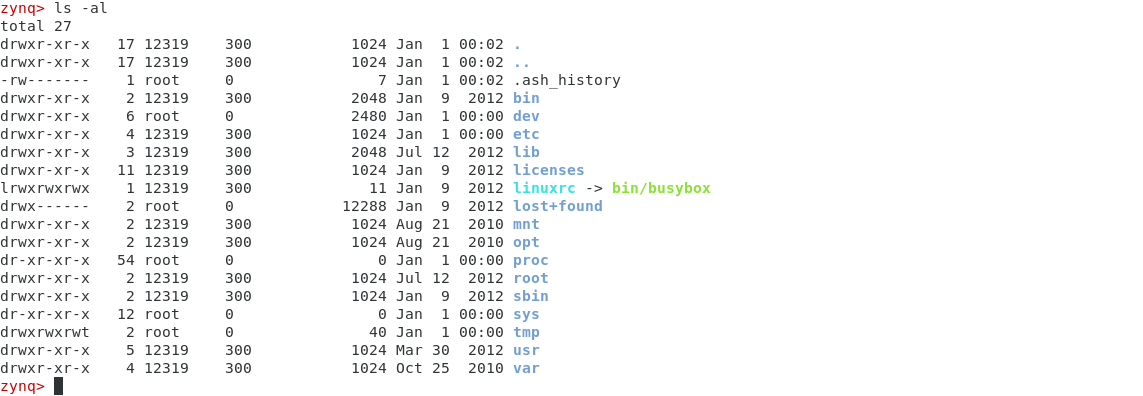
\includegraphics[width=\textwidth]{ls.png}
    \caption{ls -al output in Picocom.}
\end{figure}

After using \verb|cd <directory>| to each directory and run \verb|touch hello.txt| in each directory, I found that any directory with \verb|drwxr-xr-x| is writable. Directories with different permissions are described in the following table:

\begin{table}[ht]
\centering
\begin{tabular}{@{}lcc@{}}
\toprule
Name                              & Permission & Writable? \\ \midrule
.ash\_history                     & -rw- - - - - - - &           \\ \midrule
linuxrc $\rightarrow$ bin/busybox & lrwxrwxrwx & No        \\ \midrule
lost + found                      & drwx- - - - - - &           \\ \midrule
proc                              & dr-xr-xr-x &           \\ \midrule
sys                               & dr-xr-xr-x &           \\ \midrule
tmp                               & drwxrwxrwt & Yes       \\ \bottomrule
\end{tabular}
\caption{Linux directories whose permission is not drwxr-xr-x.}
\end{table}

% finish the table by testing permissions

After rebooting the board, all changes made to the file system and directories are list. For instance, the \textbf{.txt} files created disappear. This is because the changes are inside RAM and not written to secondary memory, i.e. the micro-SD card. RAM is volatile and after rebooting, its content is lost.

\textbf{Q: If you were to add another peripheral to your system after compiling the kernel, which of the above steps would you have to repeat? Why?}

A: 

\newpage

\begin{appendices}

\end{appendices}

\end{document}
